\documentclass[a4paper, 12pt]{report}
\usepackage[utf8]{inputenc} 	
\usepackage[frenchb,english]{babel}	
\usepackage[T1]{fontenc}	
\usepackage{times}
\usepackage[left=2.5cm,right=2.5cm,top=2.5cm,bottom=2.5cm]{geometry}
\usepackage{graphicx}
\usepackage{indentfirst}


\title{User Guide}
\author{Badges4Languages}



\begin{document}

\maketitle


\newpage
\thispagestyle{empty}
\hfill
\newpage
\addtocounter{page}{-1}

\newpage
	\setcounter{page}{1}
	\tableofcontents
	
	
\newpage
	\chapter*{Introduction}
	\addcontentsline{toc}{chapter}{Introduction}
	
	This is a User Guide which will explain you how to install and how to use our plugin Badges4Languages-plugin.\\
	
	This documentation refers to the version 1.1.0 of the code.
	





	\chapter{Installation and configuration}

	\begin{enumerate}
		\item Clone (or copy) this repository to the \textit{/wp-content/plugins/} directory;
    	\item Activate the plugin through the \textit{Plugins} menu in WordPress.
    	\item The \textit{Post Name} permalink form has to be set on the website, you can check it on the administration panel in \textit{Settings} > \textit{Permalink Settings} > \textit{Common Settings}.
	\end{enumerate}
	
	
	
	
	
	
	\chapter{Presentation}
	
		\section{User Roles}
		
		There are 4 user roles with this plugin :
	\begin{enumerate}
		\item \textit{Teacher} and \textit{Academy}, which allows a user to send badges to students (access to the plugin's submenu "Send Badges To Students");
		\item \textit{Student}, which gives no access to the plugin's menu in the administration panel;
    	\item \textit{Badge Editor}, which gives the same permissions as the Wordpress user role \textit{Editor} (that is to say to post, edit and delete posts and pages), combined with \textit{Teacher} or \textit{Academy}'s permissions.
	\end{enumerate}
	
	Automatically, the administrator have all the permissions on his website.\\
	
	If you want to create other roles or if you want to change the permissions for each role, there are 2 solutions :
	\begin{enumerate}
		\item Modify \textit{users\_roles\_and\_capabilities.php} (need some knowledge in programmation);
		\item Use a plugin, like \textit{Members} by Justin Tadlock, which lets the administrator manages easily the user roles and user capabilities (=permissions).
	\end{enumerate}
	
		\section{Badge School and Custom Taxonomies}
		
	Only a user with the role of administrator, editor, author, or Badge Editor can create a new badge (new custom post) and a new custom taxonomy (equivalent of a custom category).\\
	
	The Badge page corresponds to the certification that a user can get with Mozilla OpenBadges, therefore when the administrator/editor/author creates a badge, he has to give a title, a featured image (Badge image), and a category (Teacher/Student Level). \\
	
	It is optional, but the writer can file the custom metabox \textit{Badge Information} : he can add a link for one of the most used languages which gives more information about the certification's page.
	
	
	
	
	
	\chapter{Use}
	
		\section{Initialization (User Role : Administrator)}
		
			\subsection{Import Data to Database}
		
	Before getting a badge, the administrator (that is to say you if you have install the plugin) has to import his data into the database and to fill a form which contains his firm's information. First, when the plugin is installed and activated, the administrator has to give the list of languages and translated description in order to create the badges. He has to go into the \textit{Import Data to Database} submenu which is represented by the red 1 on the figure \ref{importDataIntoDB}.
	
	\begin{figure}[h]
		\caption{\textit{Import Data to Database} Submenu}
		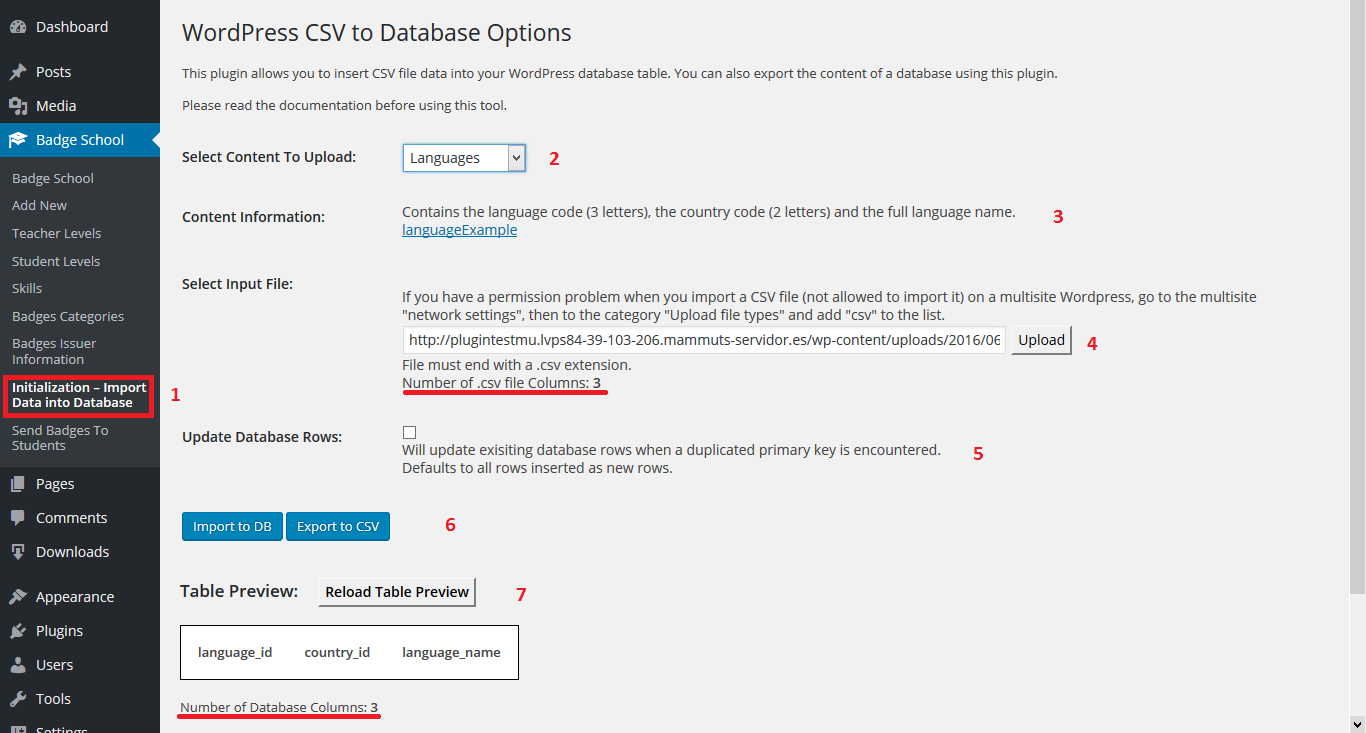
\includegraphics[scale=0.45]{includes/importDataIntoDB}
		\label{importDataIntoDB}
	\end{figure}
	
	
	Then, he chooses the kind of content he wants to add (number 2 on the figure). A short description of the selected content is displayed below, with a link to download a CSV file example (number 3). Indeed, the administrator has to give his data into a CSV file, therefore if the admin doesn't know how to use a CSV file or doesn't have a model, he can download the example and fill it. Moreover, the number of columns and the title name of columns is displayed on the \textit{Table Preview} zone (number 7).\\ 
	
	When the CSV file is complete, the user imports it by clicking on the \textit{Upload} button (number 4). A new windows opens:
	\begin{itemize}
		\item If the CSV file is on the administrator's computer, in the \textit{From Computer} tab he can import his file. When the file is loaded below, he clicks on the \textit{File URL} button and then on \textit{Insert Into Post};
		\item If the file is already on the Wordpress server (in the \textit{Media Library}), he can choose with by clicking on the \textit{Media Library} tab, then selecting \textit{All types}, and finally by clicking on \textit{File URL} and \textit{Insert Into Post}.
	\end{itemize}
	The number of columns is displayed below, so he can check that if the number of CSV file columns is the same as the Database Table Columns (number 7).\\
	
	If he has already imported data one time into one of the tables, he has to check \textit{Update Database Rows} (number 5) or he will have an error.\\
	
	If he wants to have a save of the database tables, he can export them : he selects the table (number 2) and then he clicks on \textit{Export to CSV} (number 6). \\
	
	Read the \textit{Reccurent Error} chapter if you have any problem.
	
	
	
	
	
	
	\newpage
	
			\subsection{Badges Issuer Information}
		
		The administrator has to fill the issuer's information form, or he won't be able to send certification by email. He has to go into the \textit{Badges Issuer Information} submenu which is represented by the red 1 on the figure \ref{badgesIssuerInformation}.
			
	\begin{figure}[h]
		\caption{\textit{Badges Issuer Information} Submenu}
		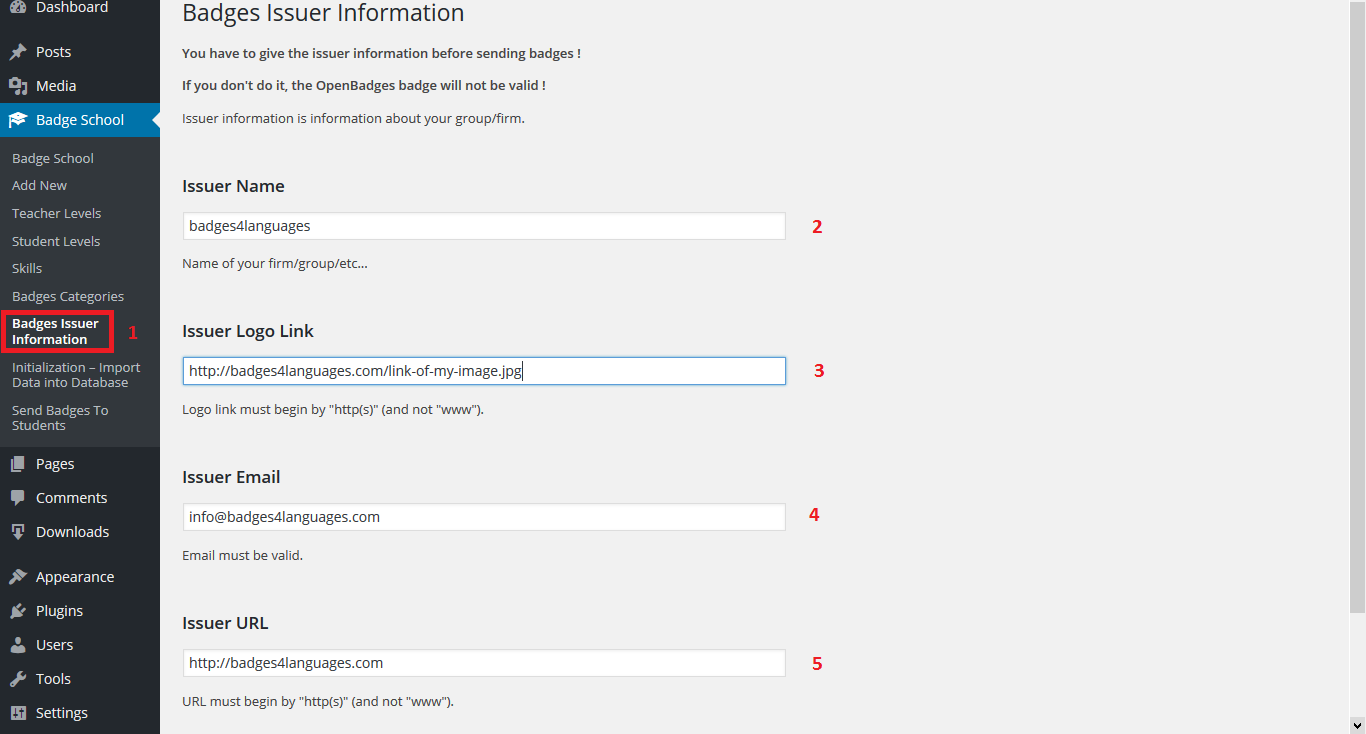
\includegraphics[scale=0.45]{includes/badgesIssuerInformation}
		\label{badgesIssuerInformation}
	\end{figure}
	
	Then, the admin gives his information into the text area (number 2 to 5). \textbf{The \textit{Issuer Logo Link} and \textit{Issuer URL} must begin by \textit{http} and not by \textit{www}} !
	
	
	
	
	\newpage
	
		\section{Sending a badge to students (User Role : Author)}
		
	A user with the role \textit{Administrator} or \textit{Author} (that is to say a teacher) can send a certification to a student(s). For example, when a student has passed an exam, he obtains a language level, so the teacher who corrected the exam has to award the student. To award a student, the teacher has to go into the \textit{Send Badges To Students} submenu which is represented by the red 1 on the figure \ref{sendBadgesToStudents}.
	
	\begin{figure}[h]
		\caption{\textit{Send Badges To Students} Submenu}
		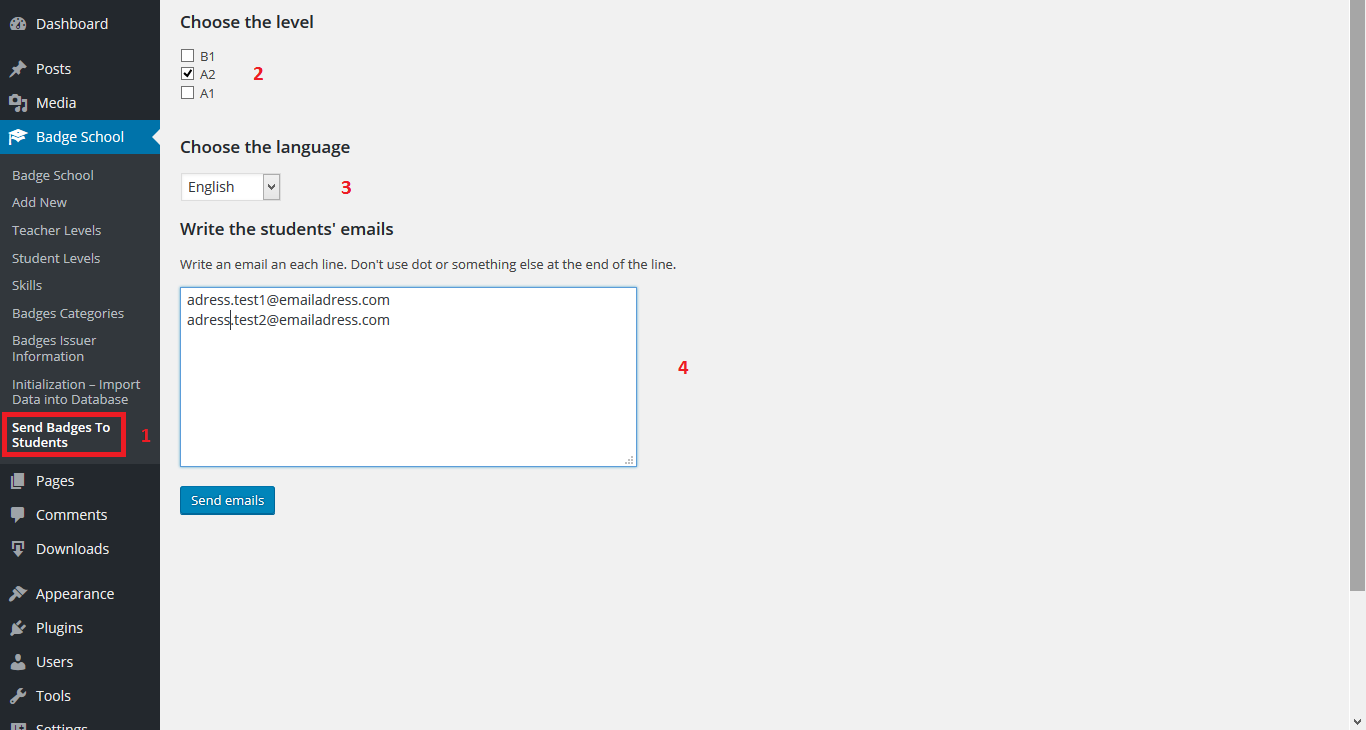
\includegraphics[scale=0.45]{includes/sendBadgesToStudents}
		\label{sendBadgesToStudents}
	\end{figure}
	
	\begin{itemize}
		\item First, the teacher chooses the level (number 2). As you can see on the screenshot, there are only 3 levels : the displayed levels correspond to the badges custom post. If the administrator has not created a post for a level, this level will not appear;
		\item Then, he elects the language (number 3). The languages can be modify by the administrator in the \textit{Import Data to Database} submenu;
		\item Finally, he writes the students' emails into the text area (number 4). He has to write one email adress by line, without adding a dot or a semicolon at the end of the line.
	\end{itemize}
		
		
		
		
		
	\newpage
	
		\section{Get a self-certification badge (User Role : User)}
	
	Every user can access a certification page to obtain information about this certification. As it is shown on the figure \ref{selfCertificationPage}, the user can choose to translate the certification's description if he can't understand english (number 1 on the figure). He can also send to himself the certification of this level, by electing the language in which he wants this certification thanks to the scrollbar menu on \textit{Choose the language that you want a certification} section (number 2 on the figure).
	
	\begin{figure}[h]
		\caption{\textit{Self-certification Badge} Page}
		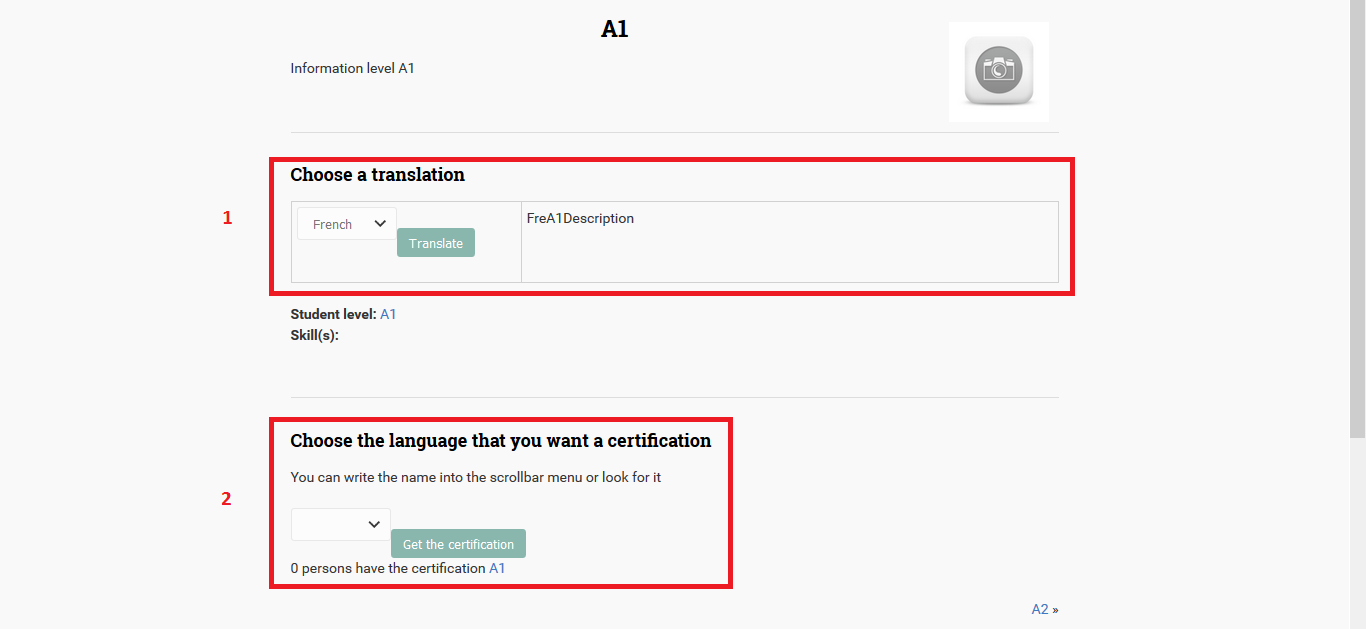
\includegraphics[scale=0.45]{includes/selfCertificationPage}
		\label{selfCertificationPage}
	\end{figure}


	Then, he will receive an email (maybe in the spam box) informing him he has just earned a Self-certification badge. By clicking on the link into the email, he will be redirect to the \textit{Accept Badge} page, which informs him he is awarded and contains a link to stock the badge in his \textit{OpenBadges Backpack}.






	\newpage
	
		\section{Shortcode : "Send Badges To Students" Page}
		
		If the administrator doesn't want that the teachers have to go the back end to send certification by email to the students, he can create a new page on his website which will contain exactly the same information as the "Send Badges To Students" plugin submenu.
		
		To do so, the administrator creates a new post (and not a new badge/new custom post !) and writes the shortcode [send\_badges] on the text field.
		
		



	\chapter{Recurrent Errors}
	
		\section{\textit{Import Data to Database} Submenu}
		
		\begin{itemize}
		
			\item You could have a permission problem when you want to import a CSV file (not allowed to import it) on a multisite Wordpress. Go to the multisite \textit{Network Settings}, then to the category \textit{Upload file types}, and add \textit{csv} to the list.

			\item When you want to import more than one CSV file into the database, you have to reload the page for each operation, otherwise it will work only for the first one;
			
			\item When you want to import for the first time data into a table, 2 bugs can appear. In those 2 cases, your data are imported, they are only visual bugs which come from another used plugin :
	 		\begin{itemize}
				\item An error message in red at the top of the page;
				\item An error message titled \textit{Internal Server Error} on a new page.
			\end{itemize}
			
		\end{itemize}
	

		\section{\textit{Badges Issuer Information} Submenu}
		
		The \textit{Issuer Logo Link} and \textit{Issuer URL} must begin by \textit{http} and not by \textit{www}
		
		\section{\textit{Accept Badge} page}
		
		When the user receives a badge by email (self-certification or sent by a teacher), he clicks on a link which redirects him to the \textit{Accept Badge} page. It could appear that the page is displayed but not the name of the badge (so you can retrieve it).
		
		To solve this problem, the administrator has to change the permalink form : he chooses \textit{Post name} or \textit{Custom Structure} in \textit{Settings} > \textit{Permalink Settings} > \textit{Common Settings}.


\end{document}